\subsection{Pengujian Citra \emph{Depth Camera} di Simulasi}
\label{subsec:citradepthsimulasi}

Pengujian citra \emph{depth camera} di simulasi dilakukan dengan cara menjalankan lingkungan \emph{indoor} pada simulator Gazebo dan menjalankan dua buah \emph{image viewer node} untuk melihat hasil penerimaan data citra berwarna dan citra kedalaman.
Seperti yang dapat dilihat pada gambar \ref{fig:rosgraphdepthcameraplugin},
  \emph{node} \lstinline{/depth_camera_plugin} akan mengirimkan \emph{topic} \lstinline{/depth_camera/image_raw} yang berisi citra berwarna ke \emph{node} \lstinline{/image_viewer_1},
  serta \emph{topic} \lstinline{/depth_camera/depth/image_raw} yang berisi citra kedalaman ke \emph{node} \lstinline{/image_viewer_2}.

\begin{figure}[ht]
  \centering
  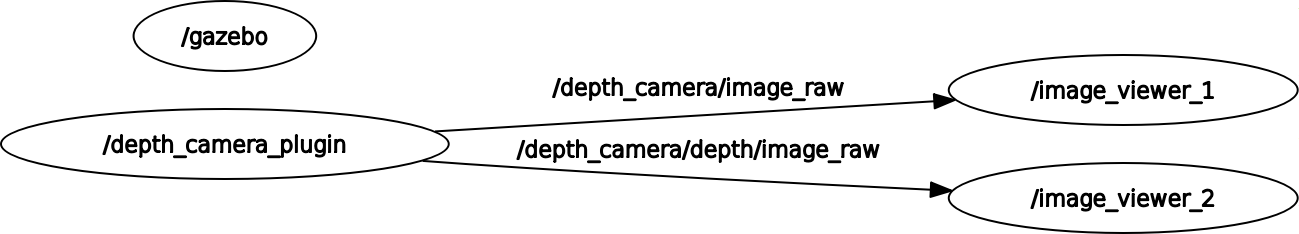
\includegraphics[width=0.95\textwidth,keepaspectratio]{gambar/rosgraph-depth-camera-plugin.png}
  \caption{Relasi antar-\emph{node} dari pengujian citra \emph{depth camera} di simulasi.}
  \label{fig:rosgraphdepthcameraplugin}
\end{figure}

Hasilnya, kedua \emph{image viewer node} tersebut akan menampilkan citra yang dikirim oleh \emph{depth camera plugin}.
Seperti yang dapat dilihat pada gambar \ref{fig:depthcamerasimulasi},
  gambar pertama menampilkan citra dari sebuah ruangan \emph{indoor} secara berwarna,
  sedangkan gambar kedua menampilkan citra dari sebuah ruangan \emph{indoor} secara hitam putih.
Citra kedua merupakan citra kedalaman, dimana semakin terang warna pada suatu pixel,
  maka jarak dari titik tersebut lebih jauh dari jangkauan kamera.

\begin{figure}[ht]
  \centering
  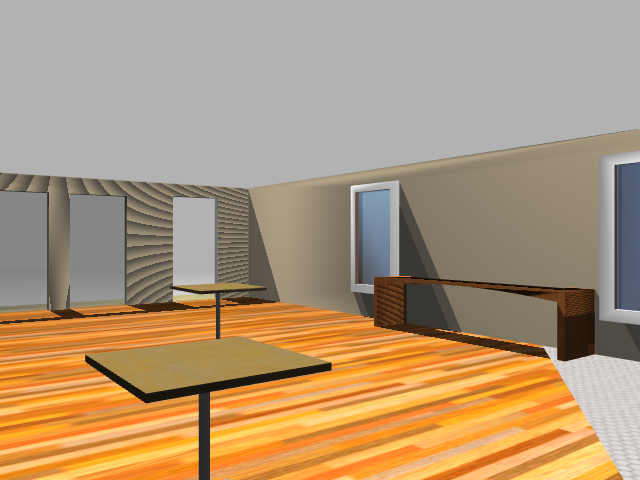
\includegraphics[width=0.4\textwidth,keepaspectratio]{gambar/citra-depth-camera-rgb-simulasi.png}
  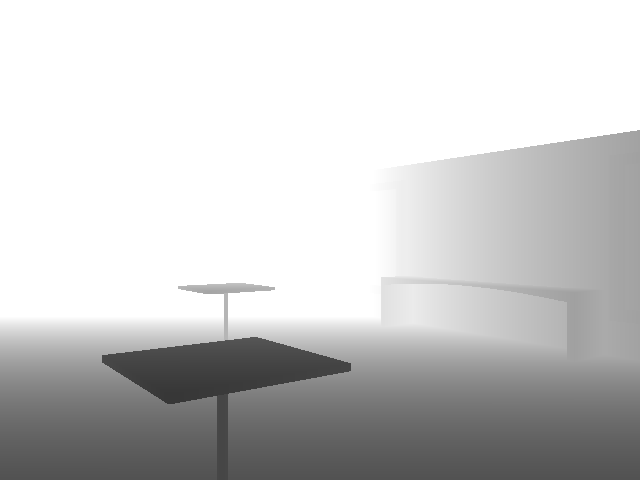
\includegraphics[width=0.4\textwidth,keepaspectratio]{gambar/citra-depth-camera-depth-simulasi.png}
  \caption{Perbandingan hasil tangkapan citra berwarna dan citra kedalaman di simulasi.}
  \label{fig:depthcamerasimulasi}
\end{figure}
